\documentclass[handout, notes=hide]{beamer}

\usepackage{attrib}
\graphicspath{{./figures/}}
\DeclareGraphicsExtensions{.pdf,.jpeg,.png,.jpg}
\usepackage[export]{adjustbox}
\usepackage{framed}

\usetheme{Rochester}
\usecolortheme{beaver}

\setbeamertemplate{bibliography entry title}{}
\setbeamertemplate{bibliography entry location}{}
\setbeamertemplate{bibliography entry note}{}

\renewcommand{\thefootnote}{\fnsymbol{footnote}}
\newcommand{\prescite}[1]{\footnote{\cite{#1}}}
\newcommand{\prestext}[1]{\footnotetext{\cite{#1}}}
\newcommand{\emaillink}[1]{\href{mailto:#1}{\nolinkurl{#1}}}
\usepackage{perpage}
\MakePerPage{footnote}

\definecolor{shadecolor}{HTML}{E8F8FF}

\begin{document}

\title{Secure Proximity-Based Identity Pairing using an Untrusted Signalling Service}
\subtitle{CCNC 2016}
\author{Tim Panton\footnotemark[1], David Llewellyn-Jones\footnotemark[2], Nathan Shone\footnotemark[3], Mahmoud Hashem Eiza\footnotemark[3]}
\institute{\footnotemark[1]Westhawk Limited, \footnotemark[2]University of Cambridge, \footnotemark[3]Liverpool John Moores University}
\date{11th January 2016}

%%%%%%%%%%%%%%%%%%%%%%%%%%%%%%%%%%%%%%%%%

\renewcommand{\thefootnote}{\arabic{footnote}}

\frame{\titlepage}
\note{
\setlength{\parskip}{0.5em}
Session is Consumer Communications and Networking, 14:00 - 15:30.

Sunset 6, Planet Hollywood, Las Vegas, NV, USA. 11th January 2016.

Talk duration is 22.5 minutes including questions (aim for 15 minutes, 8 or 9 slides).
}

\renewcommand{\thefootnote}{\fnsymbol{footnote}}

%%%%%%%%%%%%%%%%%%%%%%%%%%%%%%%%%%%%%%%%%

\begin{frame}
\frametitle{Motivation}
%\framesubtitle{}
\setlength{\parskip}{0.5em}

Provide a simple proximity-based pairing authentication mechanism to support WebRTC communication between devices

WebRTC provides a seamless way to perform P2P data streaming between devices

We'll look at IoT applications, but discuss videocalls in the paper

The WebRTC standard tackles secure data transfer, but not authentication

This leaves it open for applications to layer their own authentication approach on top

\end{frame}
\note{
\setlength{\parskip}{0.5em}
The purpose of the work is to provide a means of allowing simple, proximity-based authentication between paired devices for use with WebRTC.

The motivation for this is that WebRTC is a capable P2P protocol, but doesn't provide an authentication mechanism. Consequently some kind of P2P pairing mechanism is needed to bootstrap the WebRTC session.

As well as providing the required security/privacy property, the scheme must also integrate with the existing WebRTC standard without changes.

In the paper we discuss videocalls, but in this presentation we'll apply the protocol to IoT instead, since our focus has moved onto this as a more interesting usecase.
}

%%%%%%%%%%%%%%%%%%%%%%%%%%%%%%%%%%%%%%%%%

\begin{frame}
\frametitle{WebRTC}
\framesubtitle{Web Real Time Communications Protocol}

\begin{columns}[T]
\begin{column}[T]{0.7\textwidth}
\setlength{\parskip}{0.5em}

Developed originally by Google and now a draft W3C standard

Supported by Firefox, Chrome, Opera and Edge, used by Google Hangouts amongst others

Built using a smorgasbord of existing standards

\begin{enumerate}
\item ICE - for NAT tranversal
\item DTLS - for establishing secure sessions
\item SCTP - for data streaming
\item SRTP - for real-time streaming
\item SRTCP - for protected control messaging
\end{enumerate}

\end{column}
\begin{column}[T]{0.3\textwidth}
\vspace{2.5em}

\includegraphics[width=1.0\textwidth]{webrtc-logo-vert-retro-dist}
\end{column}
\end{columns}

\end{frame}
\note{
\setlength{\parskip}{0.5em}
Luckily the WebRTC Working Group hasn't ignored authentication entirely, which we'll come on to.

In fact, WebRTC is really a mashup of existing standards.

\begin{enumerate}
\item ICE - Interactive Connectivity Establishment
\item DTLS - Datagram Transport Layer Security
\item SCTP - Stream Control Transmission Protocol
\item SRTP - Secure Real-time Transort Protocol
\item SRTCP - Secure Real Time Control Protocol
\end{enumerate}
}

%%%%%%%%%%%%%%%%%%%%%%%%%%%%%%%%%%%%%%%%%

\begin{frame}
\frametitle{WebRTC Protocol}
\framesubtitle{An overview of the protocol}
\setlength{\parskip}{0.5em}

\centering 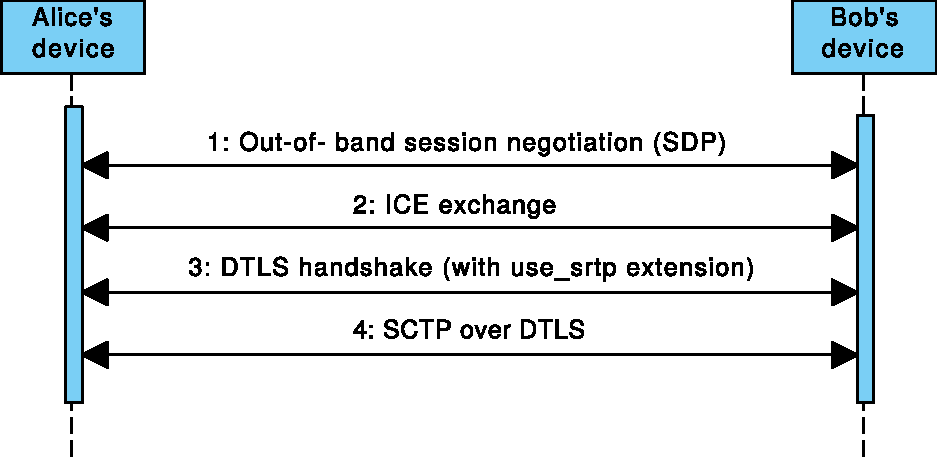
\includegraphics[width=0.9\textwidth]{webrtc-simplified}

\end{frame}
\note{
\setlength{\parskip}{0.5em}

The diagram briefly summarises how these standards work together.
\begin{enumerate}
\item WebRTC provides a means of creating the offer and response data structures, but it doesn't provide a mechanism for sharing them. That's the part we'll be focussing on.
\item The ICE exchange is for setting up the P2P connection, traversing any NATs/firewalls.
\item DTLS handshake is similar to TLS but for UDP. WebRTC only uses the handshake to establish a shared key $m$ between the two devices.
\item Once the key is established it's used to establish a secure stream between them. These can transfer any data, but the obvious types are video and audio data. For video SRTP and SRTCP would be used, but for data SCTP.
\end{enumerate}
}

%%%%%%%%%%%%%%%%%%%%%%%%%%%%%%%%%%%%%%%%%

\begin{frame}
\frametitle{Many Attractive Properties}
%\framesubtitle{}

\begin{columns}[T]
\begin{column}[T]{0.6\textwidth}
\setlength{\parskip}{0.5em}

Truly P2P, except the ICE/TURN relay

Secured against eavesdropping using UDP equivalent of TLS

Self-generated and signed certificates (no CA)

Potential for both security {\it and\/} privacy

GSOH

No mandated authentication mechanism

\end{column}
\begin{column}[T]{0.4\textwidth}
\vspace{2.5em}
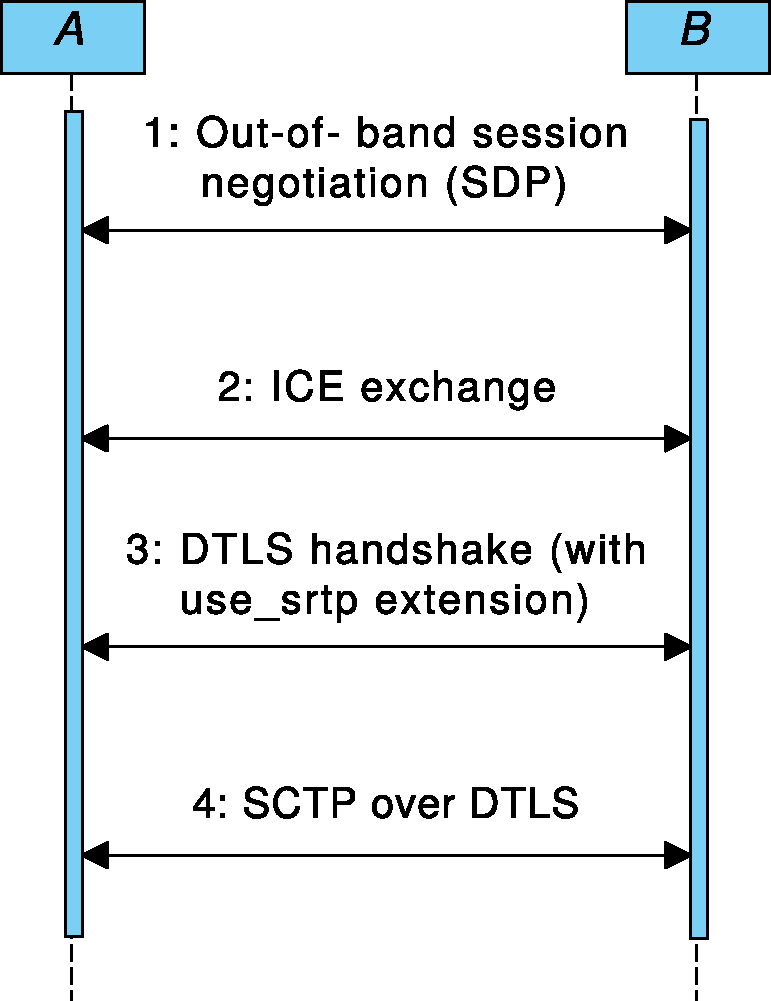
\includegraphics[width=1.0\textwidth]{webrtc-simplified-thinner}
\end{column}
\end{columns}
\end{frame}
\note{
\setlength{\parskip}{0.5em}
The figure is a reformatted version of that on the previous slide.

WebRTC is a thoughtfully considered protocol. It has many nice features.

However, the fact there's no mandated authentication mechanism means that the protocol must be bootstrapped by some other (potentially existing) mechanism.

The obvious method would be to leverage an existing relationship through a third-party service (e.g. Google+ login).

However, we want to provide a method that allows sessions to be established between devices in a way that prevents the third-party service tracking the user or violating the security.
}

%%%%%%%%%%%%%%%%%%%%%%%%%%%%%%%%%%%%%%%%%

\begin{frame}
\frametitle{Our Aims}
%\framesubtitle{}

\begin{columns}[T]
\begin{column}[T]{0.6\textwidth}
\setlength{\parskip}{0.5em}

Develop an authentication/pairing protocol between two IoT devices

Maintain security and privacy

\begin{enumerate}
\item Mutual Authentication
\item Encrypted communication
\item Prevent middle-person attacks
\item Minimise third-party trust requirements
\item Prevent correlation across streams
\end{enumerate}

\end{column}
\begin{column}[T]{0.4\textwidth}
\vspace{2.5em}
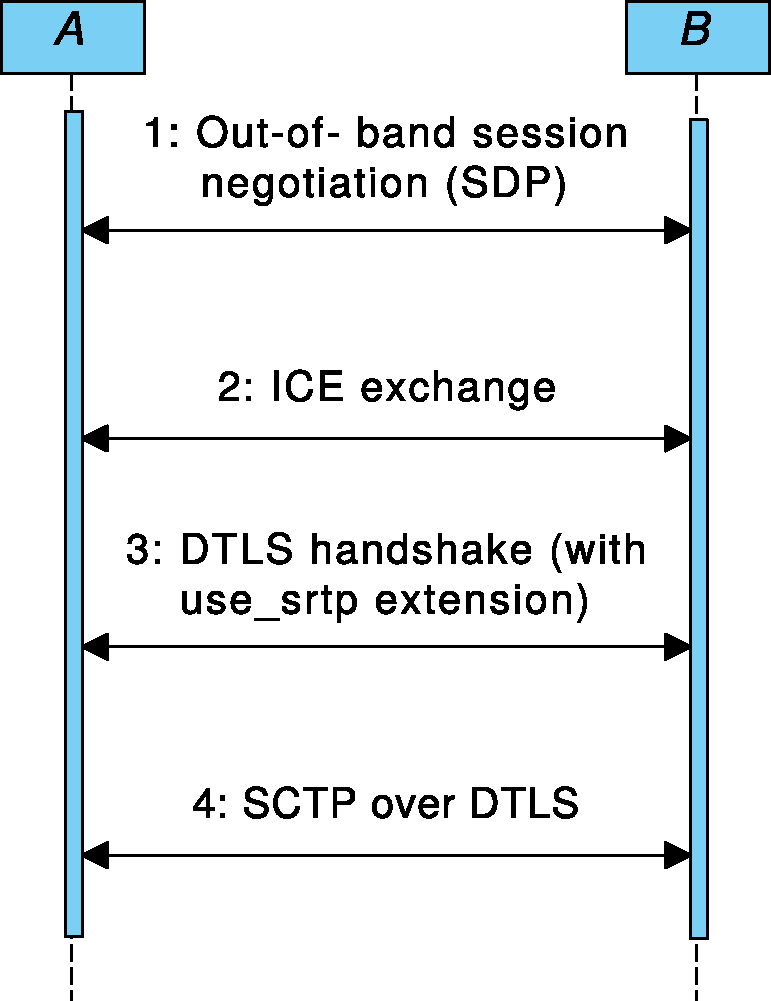
\includegraphics[width=1.0\textwidth]{webrtc-simplified-thinner}
\end{column}
\end{columns}

\end{frame}
\note{
\setlength{\parskip}{0.5em}

Our aims are therefore as shown on the slide.

To understand how we can bootstrap WebRTC it will be helpful to look at the full WebRTC protocol, including how a third party service might be used for authentication.
}

%%%%%%%%%%%%%%%%%%%%%%%%%%%%%%%%%%%%%%%%%

%%%%%%%%%%%%%%%%%%%%%%%%%%%%%%%%%%%%%%%%%

\begin{frame}
\frametitle{WebRTC Detail}
\framesubtitle{Authenticated vouched for by a third-party service}

\centering 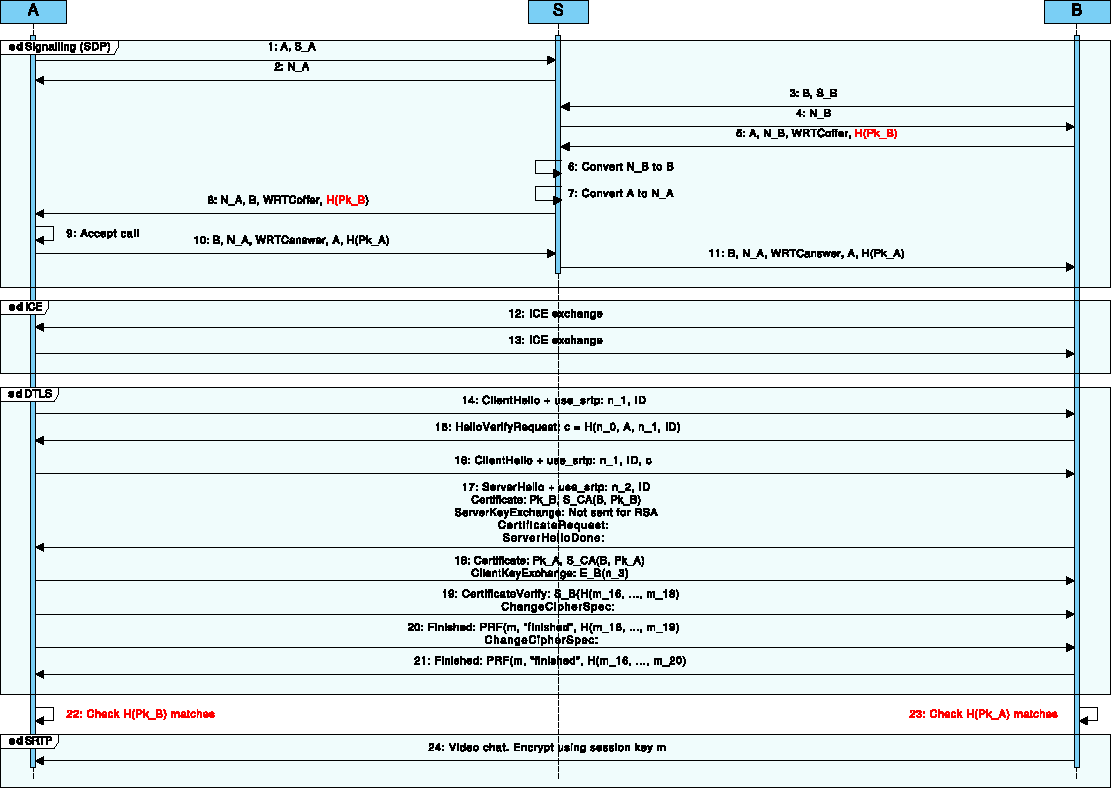
\includegraphics[width=1.0\textwidth]{webrtc}

\end{frame}
\note{
\setlength{\parskip}{0.5em}
Here we can see a full protocol sequence diagram. This is split into the same four sections (session negotiation, NAT traversal, secure session key establishment, secure streaming) as our simplified version from earlier.

The text is very small, but I've highlighted the important parts in red.

The DTLS key establishment relies on public/private key pairs. Essentially the devices authenticate themselves using RSA certificates in steps 17 and 18). From these a session key $m$ is generated using a PRF (steps 20, 21, 24).

A field is also included in the WRTCoffer for exchanging a hash of the public keys in advance (steps 5 and 8). These can then be checked after the DTLS handshake to ensure the certificates belong to the correct identities (steps 22, 23).

We want to replace steps 1-11, which here rely on a third party service we've previously authenticated to.
}

\begin{frame}
\frametitle{Pairing}
\framesubtitle{QR Code Visual Channel for asymmetric pairing}

\begin{columns}[T]
\begin{column}[T]{0.33333\textwidth}
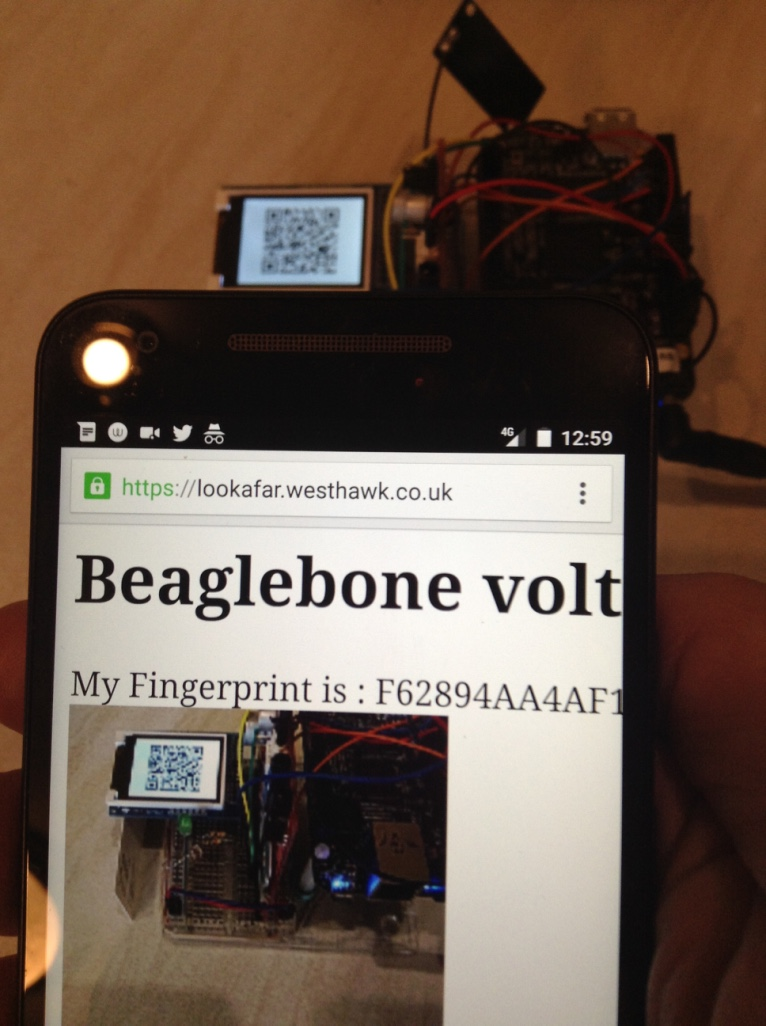
\includegraphics[width=1.0\textwidth]{iot-screen}
\end{column}
\begin{column}[T]{0.33333\textwidth}
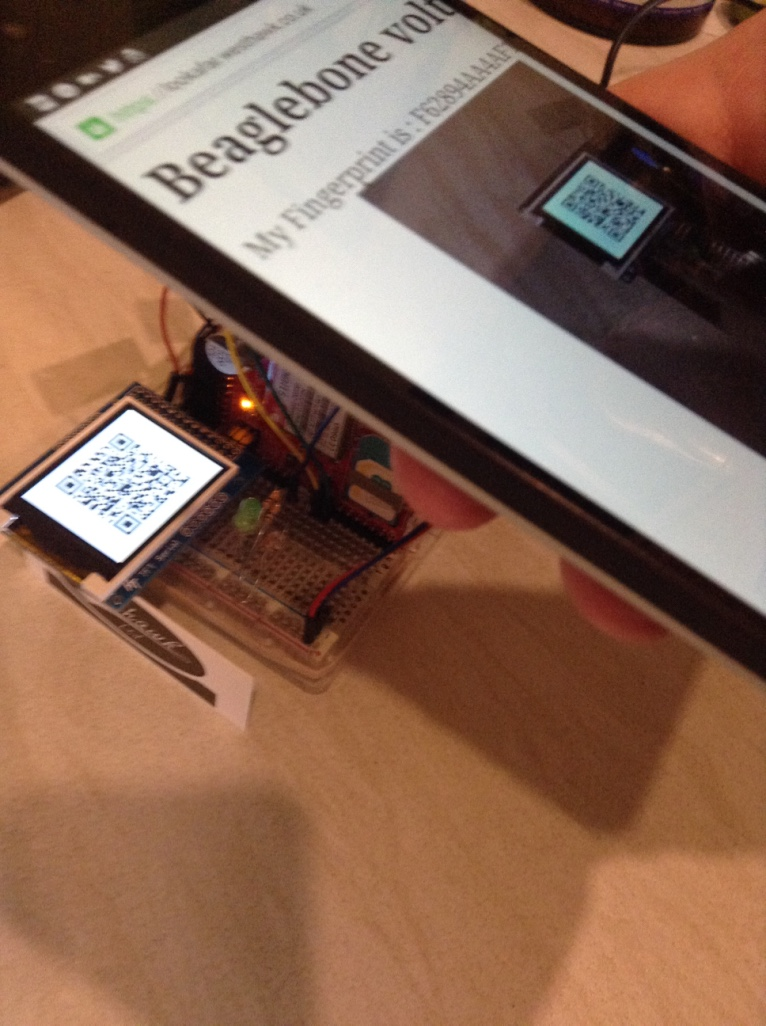
\includegraphics[width=1.0\textwidth]{iot-scan}
\end{column}
\begin{column}[T]{0.33333\textwidth}
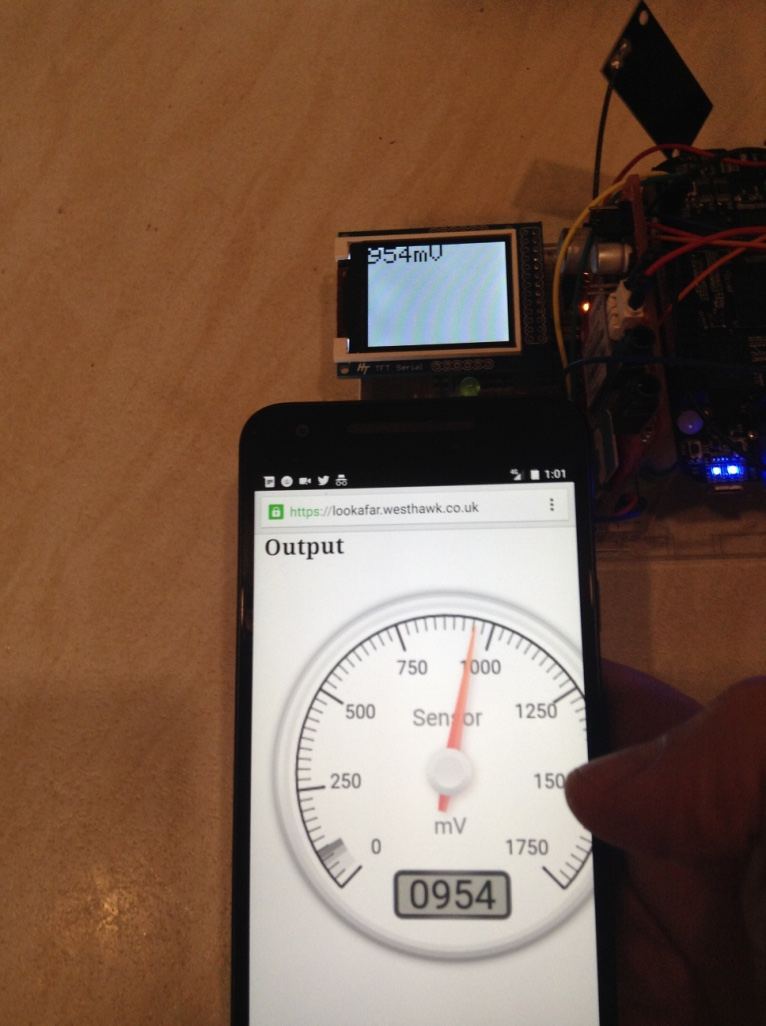
\includegraphics[width=1.0\textwidth]{iot-reading}
\end{column}
\end{columns}

\end{frame}
\note{
\setlength{\parskip}{0.5em}
Our approach uses a QR-code visual channel for the authentication step rather than the service.

In a novel step the approach avoids the need for pre-established identities by using the hash of the public keys as transient identities registered at a signalling service.

The QR code is used to provide a `secure' channel between the two devices that the user wants to pair.

From the user's point of view, they run code on both devices. On one device the code displays a QR code. On the other it provides a scanner the user scans it with.

From the user's perspective this completes the process. The photos are showing the a Beagleboard implementation that transfers voltage readings.
}

%%%%%%%%%%%%%%%%%%%%%%%%%%%%%%%%%%%%%%%%%

\begin{frame}
\frametitle{Signalling Service}
%\framesubtitle{}
\setlength{\parskip}{0.5em}

Use a third-party signalling service for message passing (e.g. \href{https://www.respoke.io}{\nolinkurl{respoke.io}})

Service provides connection

But no trust or privacy requirements

Use certificate hashes $H(Pk_A)$ and $H(Pk_B)$ as identities of $A$ and $B$

$Pk_A$ and $Pk_B$ are randomly generated.

\end{frame}
\note{
\setlength{\parskip}{0.5em}
In the background a third party signalling service is used to allow network communication between the two devices.

There should be no trust or privacy assumptions for this service, but we'll return to this in the security analysis.

The devices register their temporary identities with the signalling service, to be used just while session negotiation takes place. After this they can be de-registered (or just left).
}

%%%%%%%%%%%%%%%%%%%%%%%%%%%%%%%%%%%%%%%%%

\begin{frame}
\frametitle{Protocol Process}
%\framesubtitle{}

\centering 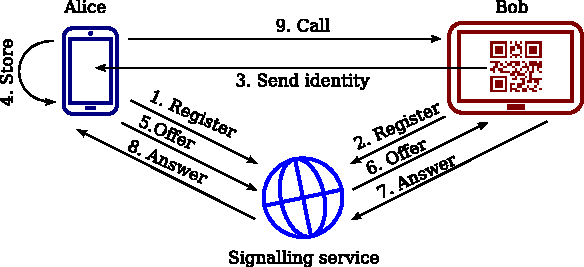
\includegraphics[width=1.0\textwidth]{interaction}

\end{frame}
\note{
\setlength{\parskip}{0.5em}

This shows the complete sequence of steps that take place.
}

%%%%%%%%%%%%%%%%%%%%%%%%%%%%%%%%%%%%%%%%%

\begin{frame}
\frametitle{Protocol Sequence}
%\framesubtitle{}

\centering 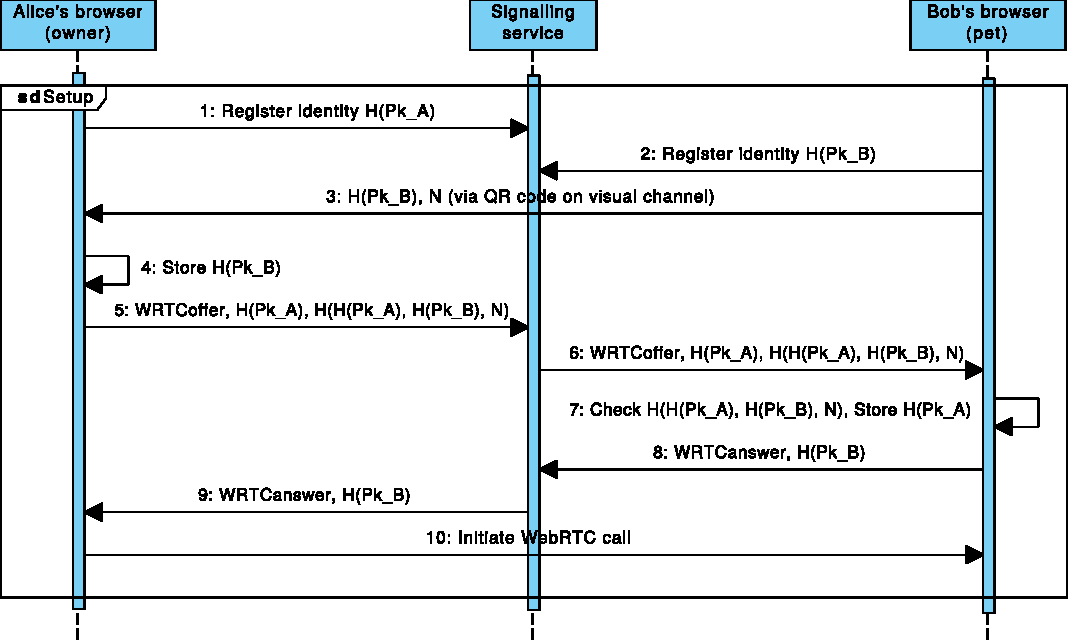
\includegraphics[width=1.0\textwidth]{core-qr}

\end{frame}
\note{
\setlength{\parskip}{0.5em}
This shows the same, but including message contents.

Note that step 3 uses the visual QR code channel. All other steps use internet comms.

The WRTCoffer and WRTCanswer structures are used for stream negotiation and are defined by WebRTC.

Note the use of $H(Pk_A)$ and $H(Pk_B)$ for the identities registered at the signalling service.

On the remaining slides we'll consider the security characteristics of the protocol.
}

%%%%%%%%%%%%%%%%%%%%%%%%%%%%%%%%%%%%%%%%%

\begin{frame}
\frametitle{Security Analysis}
\framesubtitle{Mutual Authentication}

\begin{columns}[T]
\begin{column}[T]{0.6\textwidth}
%\setlength{\parskip}{0.5em}

Authentication from $B$ to $A$
\begin{enumerate}
\item Transfer $H(Pk_B)$ at step 3 using QR code
\item Attacker capturing $H(Pk_B)$ can't use it in step 3
\end{enumerate}

Authentication $A$ to $B$
\begin{enumerate}
\item Sent over open channel in steps 5-6
\item $S$ can attempt middle-person attack
\item Challenge $N$ achieves integrity
\item Replay attack mitigated by freshness of $N$
\end{enumerate}


\end{column}
\begin{column}[T]{0.4\textwidth}
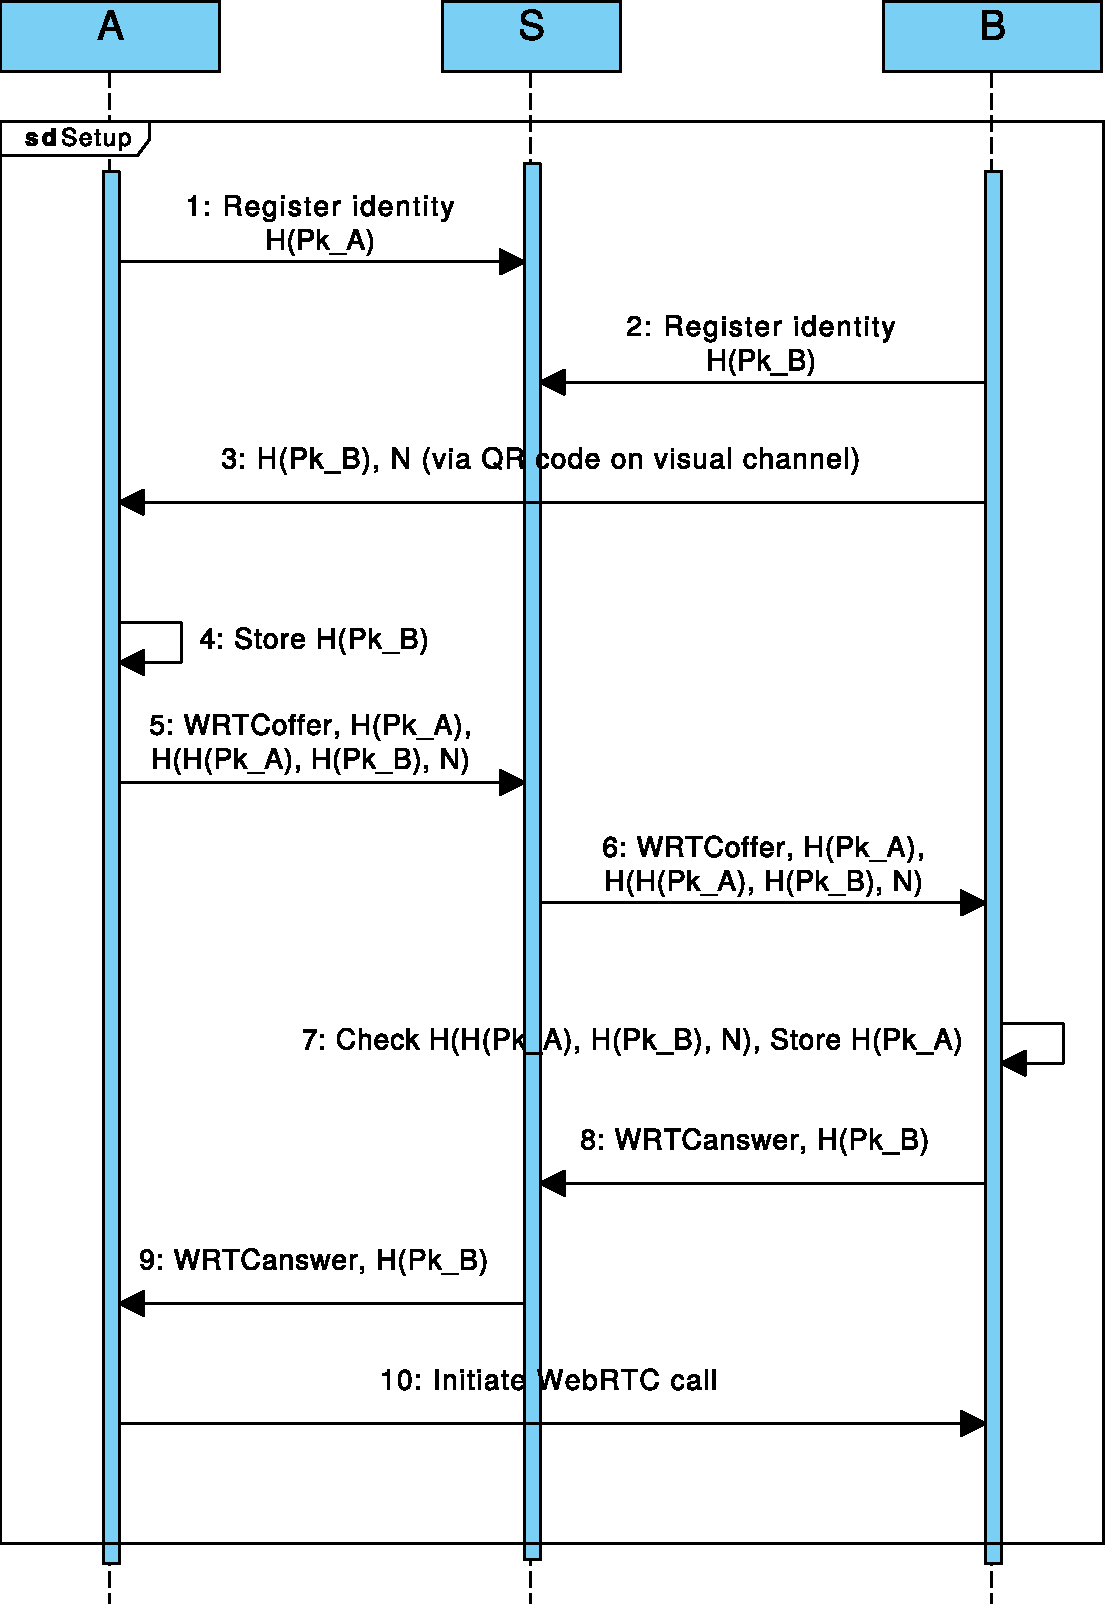
\includegraphics[width=1.0\textwidth]{core-qr-thin}
\end{column}
\end{columns}

\end{frame}
\note{
\setlength{\parskip}{0.5em}
The figure is a reformatted version of that on the previous slide.

We need mutual authentication, but does this achieve it?

Identities of $A$ and $B$ sent in the clear in steps 1 and 2.

We have to make some reasonable assumptions about the security of the QR code channel in step 3. In particular, our threat model assumes the two devices are trusted (not compromised) and that the code running on each device can be trusted (e.g. it can be checked on the device).
}

%%%%%%%%%%%%%%%%%%%%%%%%%%%%%%%%%%%%%%%%%

\begin{frame}[fragile]
\frametitle{Security Analysis}
\framesubtitle{Middle-Person Attacks}

\begin{columns}[T]
\begin{column}[T]{0.6\textwidth}
\setlength{\parskip}{0.5em}
Have achieved mutual authentication

No middle-person attack to step 7

WRTCanswer integrity not protected
\begin{enumerate}
\item Must match WRTCoffer
\item Susceptible to downgrade attack
\end{enumerate}
\setlength{\fboxrule}{10.0em}
\begin{snugshade}
\begin{tiny}
\begin{verbatim}{"type":"answer","sdp":"
v=0
o=mozilla...THIS_IS_SDPARTA-41.0.1 4104634441...
s=-
t=0 0
a=sendrecv
a=fingerprint:sha-256 BF:3E:50:AE:15:FF:5E:D8...
a=group:BUNDLE sdparta_0
a=ice-options:trickle
..."}
\end{verbatim}
\end{tiny}
\end{snugshade}

\end{column}
\begin{column}[T]{0.4\textwidth}
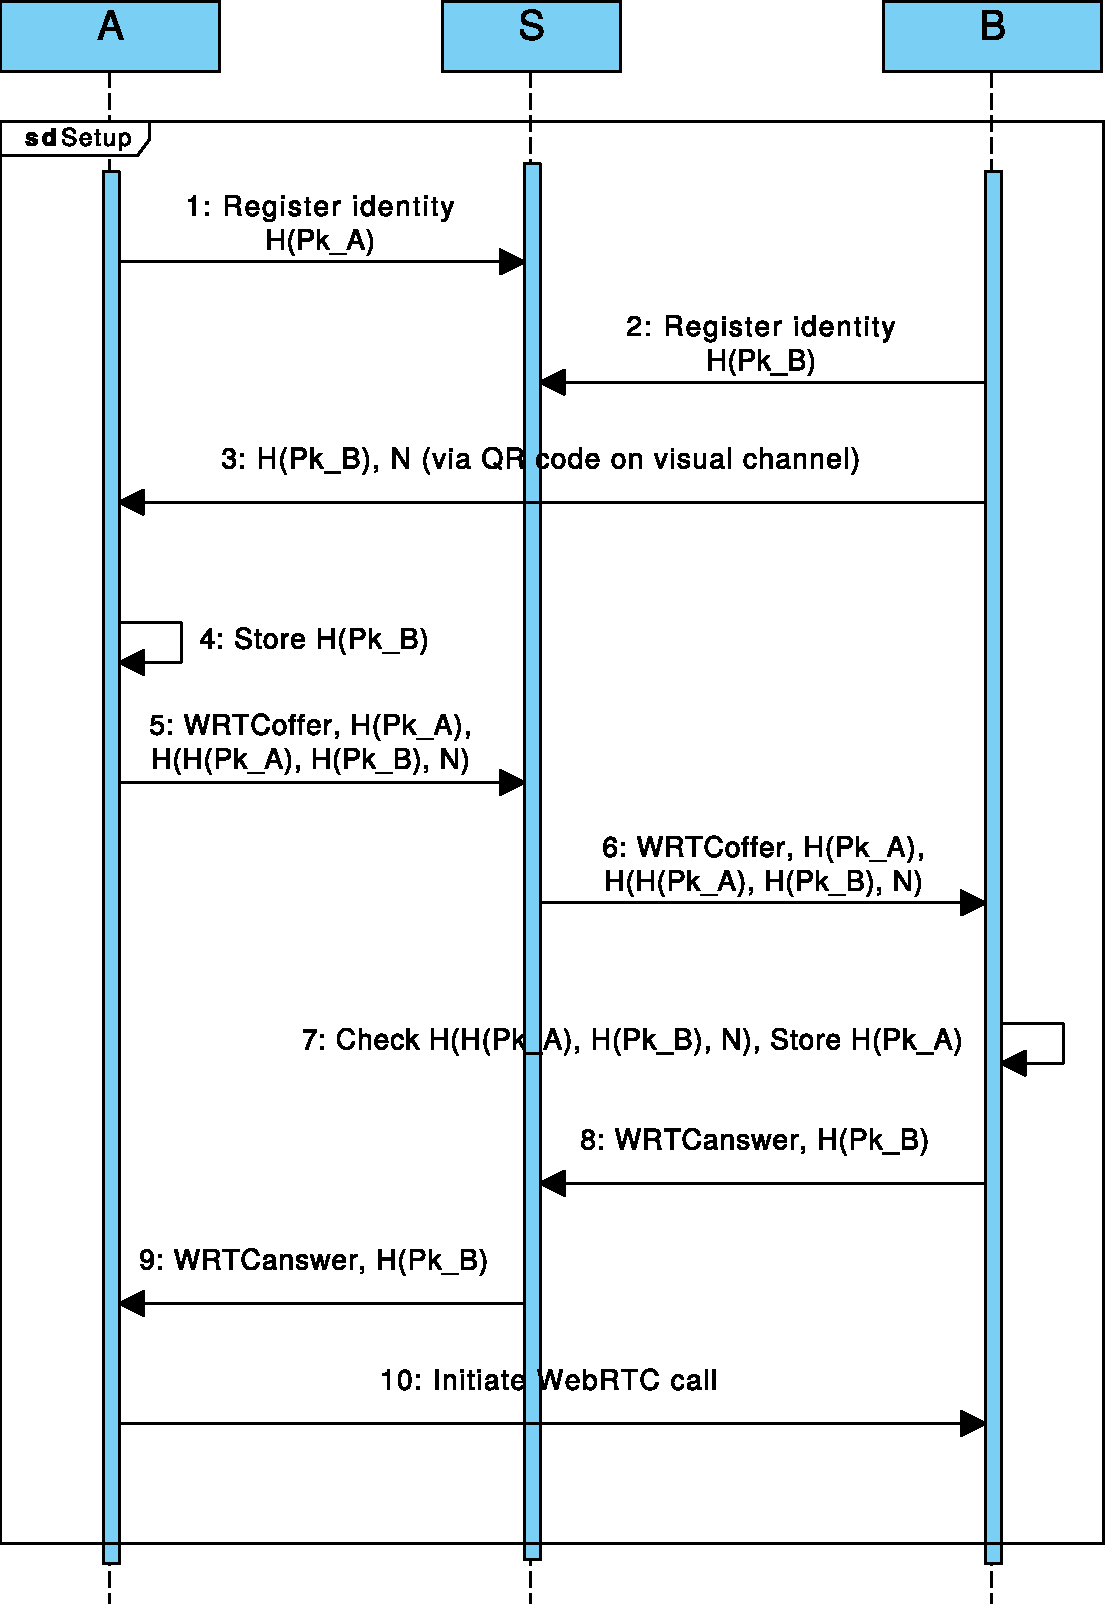
\includegraphics[width=1.0\textwidth]{core-qr-thin}
\end{column}
\end{columns}
\end{frame}
\note{
\setlength{\parskip}{0.5em}

Can a middle-person attack successfully allow eavesdropping or session-hijacking?

This is particularly important since $S$ is in an ideal position to pull off such an attack.

There is a potential weakness with the integrity of the WRTCanswer data structure, which could leave it susceptible to a downgrade attack if an attacker were to change or replace the contents.
}

%%%%%%%%%%%%%%%%%%%%%%%%%%%%%%%%%%%%%%%%%

\begin{frame}
\frametitle{Security Analysis}
\framesubtitle{Visual Channel Attacks}

\begin{columns}[T]
\begin{column}[T]{0.6\textwidth}
\setlength{\parskip}{0.5em}

Relay/replay phishing
\begin{enumerate}
\item QR code switched at step 3
\item $A$ pairs with attacker's device
\item Mitigated by use of trusted devices
\item Requires device integrity
\end{enumerate}

Relay hijack
\begin{enumerate}
\item Attacker captures code at step 3
\item Attacker pairs with $B$ before $A$
\item Visual channel assumed private
\end{enumerate}

\end{column}
\begin{column}[T]{0.4\textwidth}
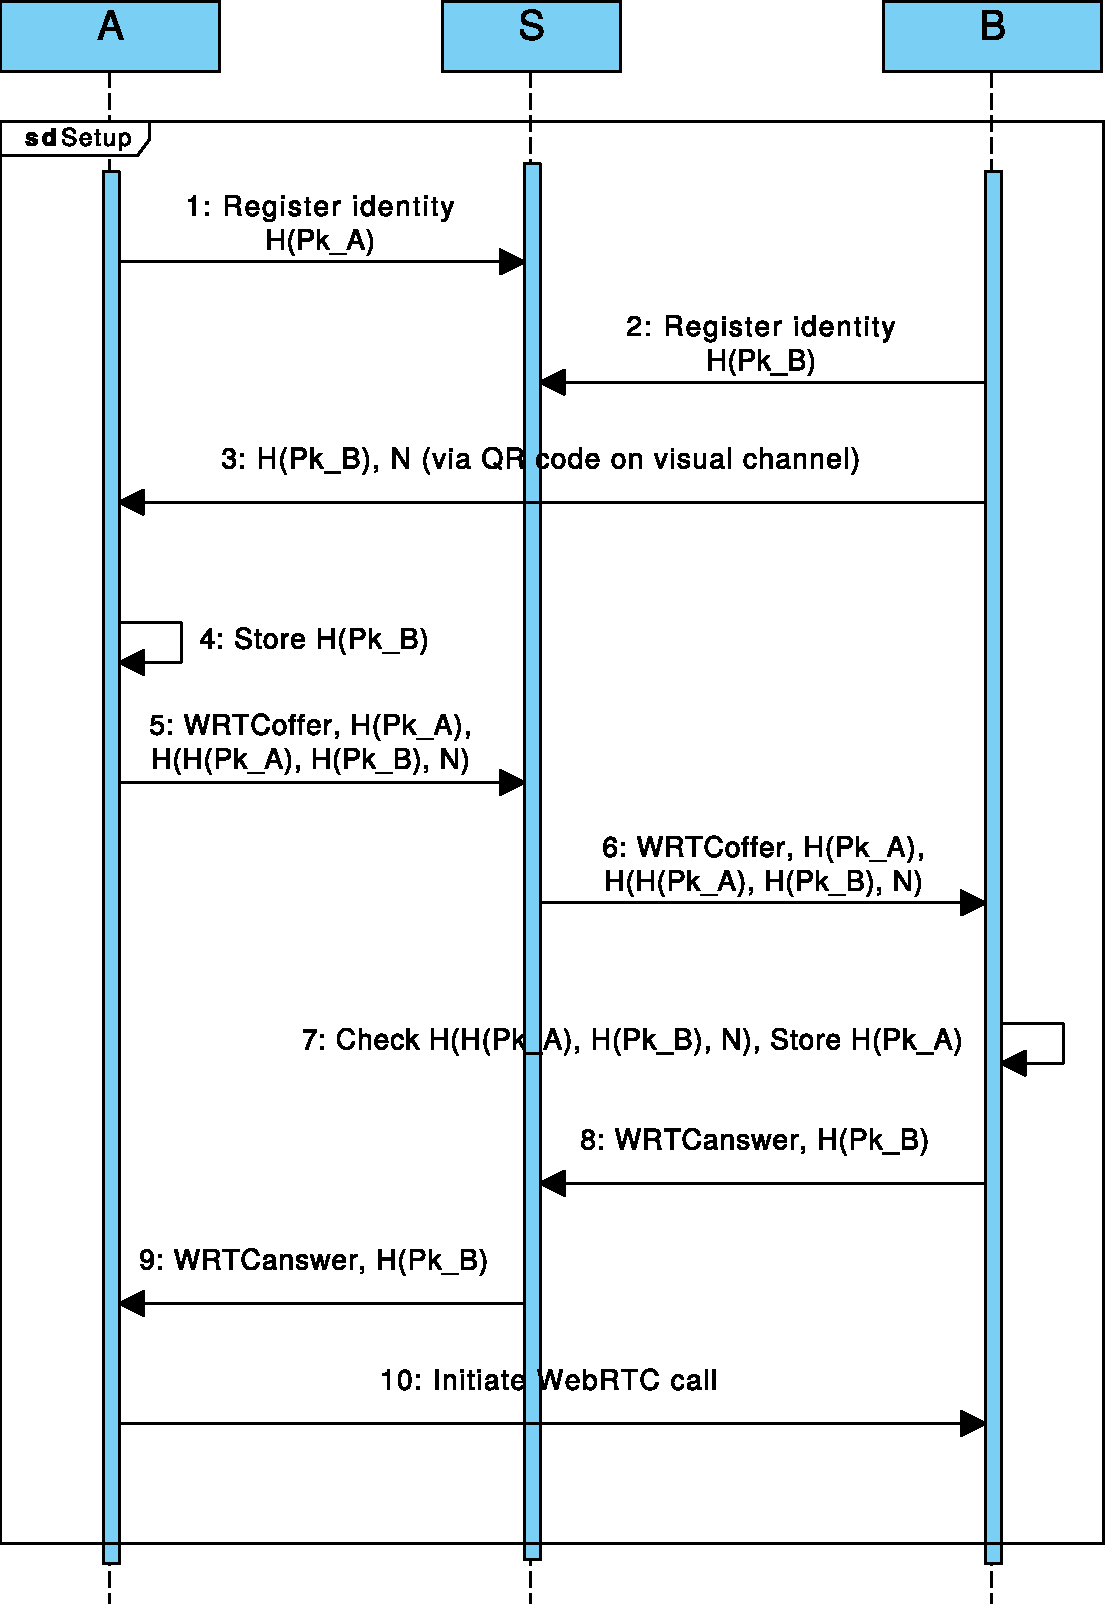
\includegraphics[width=1.0\textwidth]{core-qr-thin}
\end{column}
\end{columns}
\end{frame}
\note{
\setlength{\parskip}{0.5em}

Our attacker model assumes the visual channel to be secure, but this won't prevent an attacker requesting a QR code and reusing it.

Is there any potential for relay and replay attacks? These could have one of two outcomes. Either the user could be tricked into connecting to the wrong device, or an attacker could hijack the process, causing a similar result.

The result would be the user ends up streaming data to/from the attacker's device, rather than the intended device.
}

%%%%%%%%%%%%%%%%%%%%%%%%%%%%%%%%%%%%%%%%%

\begin{frame}
\frametitle{Security Analysis}
\framesubtitle{Signalling Server Trust}

\begin{columns}[T]
\begin{column}[T]{0.6\textwidth}
\setlength{\parskip}{0.5em}

Want to minimise trust

Assume $S$ is a malicious middle-person

$S$ only needed during signalling, not for data streaming

Attacker can correlate calls between pairs, but not across distinct pairs except by IP address

\end{column}
\begin{column}[T]{0.4\textwidth}
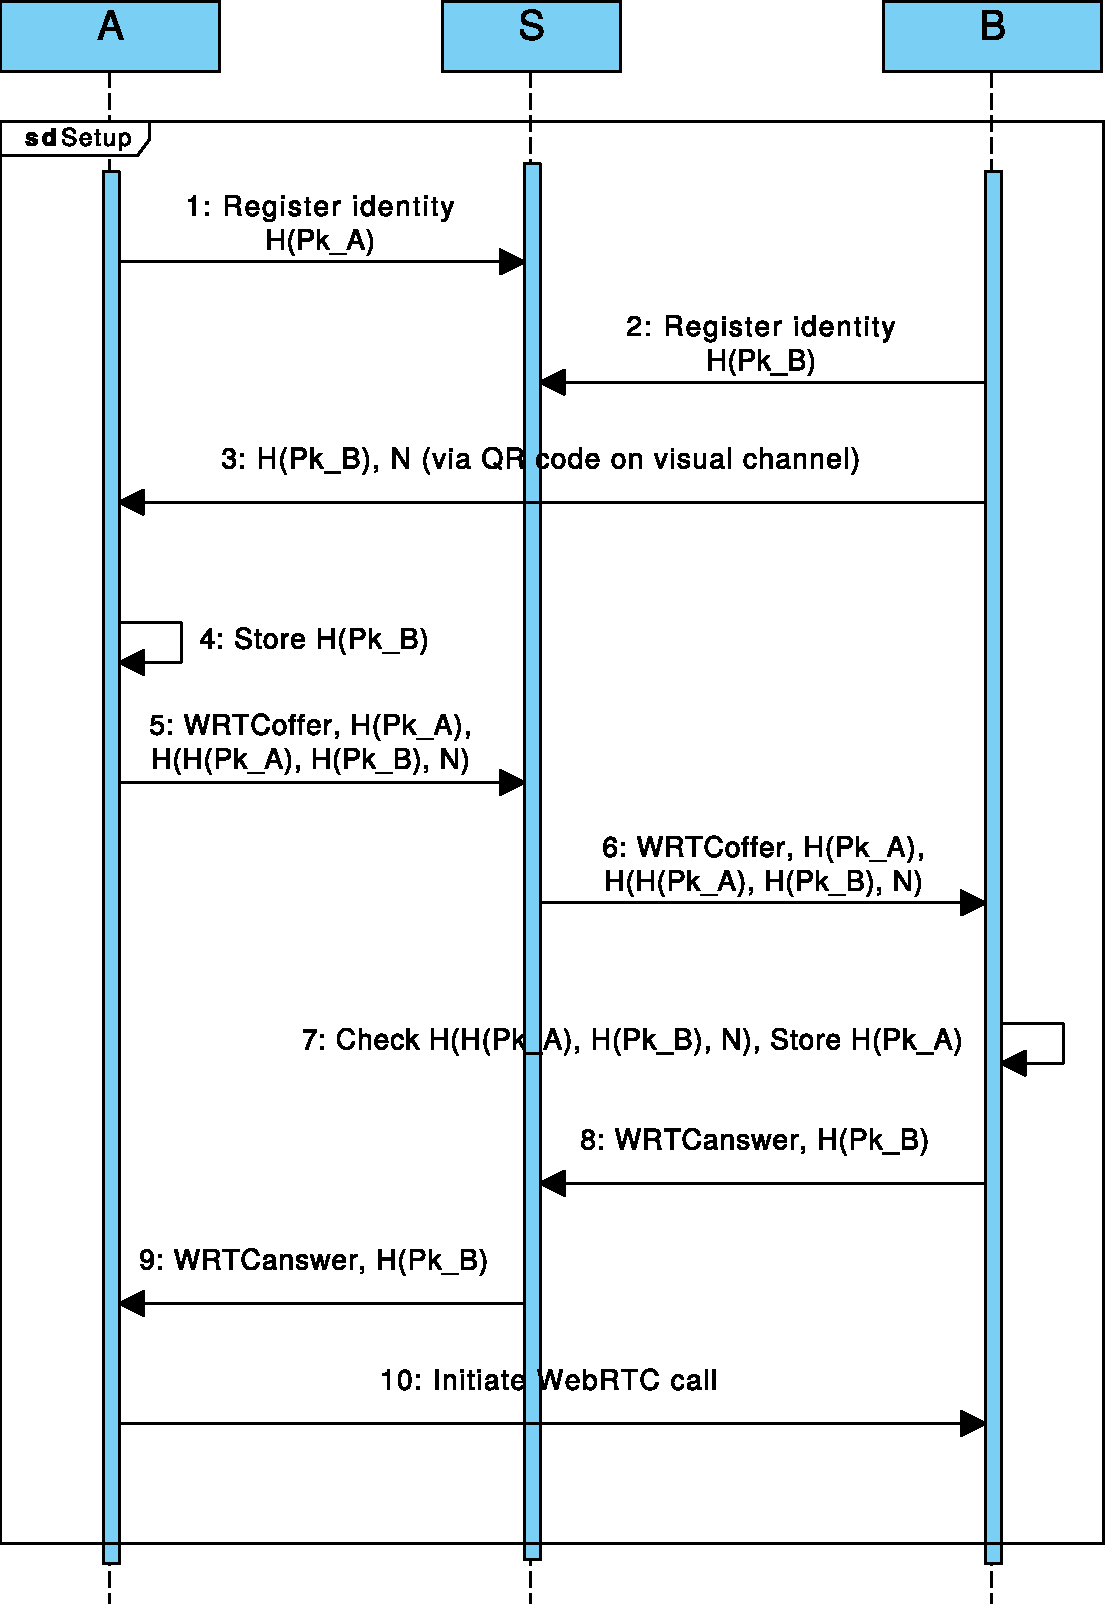
\includegraphics[width=1.0\textwidth]{core-qr-thin}
\end{column}
\end{columns}
\end{frame}
\note{
\setlength{\parskip}{0.5em}

The Signalling Service is needed to work around NATs and firewalls. Otherwise it could be removed.
}

%%%%%%%%%%%%%%%%%%%%%%%%%%%%%%%%%%%%%%%%%

\begin{frame}
\frametitle{Conclusion}
\setlength{\parskip}{0.5em}

Conclusion
\begin{enumerate}
\item Satisfies security requirements
\item Provides security and privacy
\item Integrates seemlessly with WebRTC
\end{enumerate}

Future Work
\begin{enumerate}
\item Formal analysis using Strand-Spaces or BAN logic
\item Explore IoT application space
\item Usability testing
\end{enumerate}

\end{frame}
\note{
\setlength{\parskip}{0.5em}

BAN logic - Burrows-Abadi-Needham logic
}

%%%%%%%%%%%%%%%%%%%%%%%%%%%%%%%%%%%%%%%%%

\begin{frame}
\frametitle{Fin}
Try it yourself at \url{yopet.us}
\setlength{\parskip}{1.0em}

Tim Panton, Westhawk Limiated \\
\emaillink{thp@westhawk.co.uk}

David Llewellyn-Jones, University of Cambridge \\
\emaillink{David.Llewellyn-Jones@cl.cam.ac.uk}

Nathan Shone, Liverpool John Moores University \\
\emaillink{N.Shone@ljmu.ac.uk}

Mahmoud Hashem Eiza, Liverpool John Moores University \\
\emaillink{M.Hashemeiza@ljmu.ac.uk}

\end{frame}
\note{
\setlength{\parskip}{0.5em}

Thanks for listening! Rapturous applause!
}

%%%%%%%%%%%%%%%%%%%%%%%%%%%%%%%%%%%%%%%%%

%\begin{frame}
%\frametitle{Bibliography}
%{\tiny
%\bibliographystyle{apalike}
%\bibliography{main}
%}%
%\end{frame}

%%%%%%%%%%%%%%%%%%%%%%%%%%%%%%%%%%%%%%%%%

\end{document}
